\documentclass[10pt]{beamer}
\usefonttheme{professionalfonts}
%\usetheme{CambridgeUS}
%
% Choose how your presentation looks.
%
% For more themes, color themes and font themes, see:
% http://deic.uab.es/~iblanes/beamer_gallery/index_by_theme.html
%
\mode<presentation>
{
  \usetheme{default}      % or try Darmstadt, Madrid, Warsaw, ...
  \usecolortheme{beaver} % or try albatross, beaver, crane, ...
  \usefonttheme{default}  % or try serif, structurebold, ...
  \setbeamertemplate{navigation symbols}{}
  \setbeamertemplate{caption}[numbered]
} 

\usepackage[english]{babel}
\usepackage[utf8x]{inputenc}
\usepackage{tikz}
\usepackage{pgfplots}
\usepackage{array}  % for table column M
\usepackage{makecell} % to break line within a cell
\usepackage{verbatim}
\usepackage{graphicx}
\usepackage{epstopdf}
\usepackage{amsfonts}
\usepackage{xcolor}
\usepackage{ifthen}
%\usepackage{mathtools}
\usepackage[makeroom]{cancel}
\usetikzlibrary{spy}
%\captionsetup{compatibility=false}
%\usepackage{dsfont}
\usepackage[absolute,overlay]{textpos}
\usetikzlibrary{calc, angles,quotes}
\usetikzlibrary{pgfplots.fillbetween, backgrounds}
\usetikzlibrary{positioning}
\usetikzlibrary{arrows}
\usetikzlibrary{pgfplots.groupplots}
\usetikzlibrary{arrows.meta}
\usetikzlibrary{plotmarks}
\usetikzlibrary{decorations.markings}
\usepgfplotslibrary{groupplots}
\pgfplotsset{compat=newest} 
%\pgfplotsset{plot coordinates/math parser=false}

\usepackage{hyperref}
\hypersetup{
    colorlinks=true,
    linkcolor=blue,
    filecolor=magenta,      
    urlcolor=cyan,
}

%
%\def\EXTERNALIZE{1}
%%% Externalizing
\usepgfplotslibrary{external} 
\ifdefined\EXTERNALIZE
	\makeatletter	
	\newcommand*{\overlaynumber}{\number\beamer@slideinframe}
	\tikzset{
		beamer externalizing/.style={%
			execute at end picture={%
				\tikzifexternalizing{%
					\ifbeamer@anotherslide
					\pgfexternalstorecommand{\string\global\string\beamer@anotherslidetrue}%
					\fi
				}{}%
			}%
		},
		external/optimize=false
	}
	\let\orig@tikzsetnextfilename=\tikzsetnextfilename
	\renewcommand\tikzsetnextfilename[1]{\orig@tikzsetnextfilename{#1-\overlaynumber}}
	\makeatother
	
	\tikzset{every picture/.style={beamer externalizing}}
	
	\tikzexternalize[prefix=external/]
\fi

%%% Page numbering
\usepackage{etoolbox} % necessary for excluding beamer-only frames from page numbering

\makeatletter
\pretocmd{\beamer@@@@frame}{\alt<#1>{}{\beamer@noframenumberingtrue}}{}{}
\makeatother

\addtobeamertemplate{navigation symbols}{}{%
	\usebeamerfont{footline}%
	\usebeamercolor[fg]{footline}%
	\hspace{1em}%
	\scriptsize\insertframenumber/\inserttotalframenumber
}
%%%

% For circular convolution
\newcommand\encircle[1]{%
	\tikz[baseline=(X.base)] 
	\node (X) [anchor=south, draw, shape=circle, inner sep=0mm, align=center] {\scriptsize\strut #1};}

\definecolor{matlabcomment}{RGB}{34,139,34}

\pgfmathdeclarefunction{gauss}{1}{%
	\pgfmathparse{1/(sqrt(2*pi))*exp(-((#1)^2)/2)}%
}

\pgfmathdeclarefunction{sign}{1}{%
	\pgfmathparse{1*(#1 > 0) - 1*(#1 < 0)}%
}

\pgfmathdeclarefunction{laplacian}{2}{%
	\pgfmathparse{1/(#2*2)*exp(-(abs(x-#1))/(#2))}%
}

\pgfmathdeclarefunction{pretty_func}{1}{%
	\pgfmathparse{cos(deg(#1/2)) - sin(deg(#1)) + cos(deg(#1/2)-45) - sin(deg(#1/4)-154)}%
}

\pgfplotsset{
	dirac/.style={
		mark=triangle*,
		mark options={scale=2},
		ycomb,
		scatter,
		visualization depends on={y/abs(y)-1 \as \sign},
		scatter/@pre marker code/.code={\scope[rotate=90*\sign,yshift=-2pt]}
	}
}

\def\thickness{very thick}

\tikzset{
amark/.style 2 args={
	decoration={             
		markings, 
		mark=at position {0.5} with { 
			\arrow{stealth},
			\node[#2] {#1};
		}
	}, \thickness,
	postaction={decorate}
},
earlymark/.style 2 args={
	decoration={             
		markings, 
		mark=at position {0.25} with { 
			\arrow{stealth},
			\node[#2] {#1};
		}
	}, \thickness,
	postaction={decorate}
},
latemark/.style 2 args={
	decoration={             
		markings, 
		mark=at position {0.8} with { 
			\arrow{stealth},
			\node[#2] {#1};
		}
	}, \thickness,
	postaction={decorate}
},
zpath/.style={
	decoration={             
		markings, 
		mark=at position {0.5} with { 
			\arrow{stealth},
			\node[#1] {$z^{-1}$};
		}
	}, \thickness,
	postaction={decorate}
},
terminal/.style 2 args={draw,circle,inner sep=2pt,label={#1:#2}},
}


\tikzset{
	invisible/.style={opacity=0},
	visible on/.style={alt={#1{}{invisible}}},
	alt/.code args={<#1>#2#3}{%
		\alt<#1>{\pgfkeysalso{#2}}{\pgfkeysalso{#3}} % \pgfkeysalso doesn't change the path
	},
}

\newcommand\PlotSampledSpectrum[4]{%
	\def\fs{#2}%
	\def\fmax{#3}%
	\def\ros{#4}%
	\input{#1}%
}

\pgfmathdeclarefunction{invgauss}{2}{%
	\pgfmathparse{sqrt(-2*ln(#1))*cos(deg(2*pi*#2))}%
}

\pgfmathdeclarefunction{triang}{2}{%
	\pgfmathparse{(1/#2)*(#1 + #2)*and(#1 <= 0, #1 >= -#2) + (1/#2)*(-#1 + #2)*and(#1 > 0, #1 <= #2)}%
}

\pgfmathdeclarefunction{rect}{2}{%
	\pgfmathparse{and(#1 >= 0, #1 < #2)}%
}

\pgfmathdeclarefunction{dsinc}{2}{%
	\pgfmathparse{(and(#1 != 0, 1)*(sin(deg(#1*#2/2))/sin(deg(#1/2))) + and(#1 == 0, 1) * (#2)}%
}

\tikzset{
	declare function={
		sinc(\x) = (and(\x!=0, 1) * (sin(deg(pi*\x))/(pi*\x)) +
		(and(\x==0, 1) * 1);
	}
}

\DeclareMathOperator{\E}{\mathbb{E}} % expectation

\newcolumntype{M}[1]{>{\centering\arraybackslash}m{#1}}

\definecolor{blue2}{RGB}{51, 105, 232}  
\definecolor{red2}{RGB}{213, 15, 37}  
\definecolor{green2}{RGB}{0, 153, 37}  
\definecolor{green3}{rgb}{0.1922, 0.6392, 0.3294}% 
\definecolor{yellow2}{RGB}{238, 178, 17} 
\definecolor{gray2}{RGB}{102, 102, 102}
\definecolor{orange2}{RGB}{230, 85, 13}

% Qualitative pallete set1 from www.ColorBrewer.org
\definecolor{Qred}{RGB}{228,26,28}
\definecolor{Qblue}{RGB}{55,126,184}
\definecolor{Qgreen}{RGB}{77,175,74}
\definecolor{Qpurple}{RGB}{152,78,163}
\definecolor{Qorange}{RGB}{255,127,0}
\definecolor{Qyellow}{RGB}{255,255,51}
\definecolor{Qbrown}{RGB}{166,86,40}
\definecolor{Qpink}{RGB}{247,129,191}
\definecolor{Qgray}{RGB}{153,153,153}

\newcommand\SimpleSys[4]{%
	\def\xin{#2}%
	\def\Hz{#3}%
	\def\yout{#4}
	\input{#1}%
}

\newcommand\PlotExp[5]{%
	\def\A{#2}%
	\def\Legend{#3}%
	\def\ymin{#4}
	\def\ymax{#5}
	\input{#1}%
}

\newcommand\PlotSinc[5]{%
	\def\xmin{#2}%
	\def\xmax{#3}%
	\def\samples{#4}
	\def\w{#5}
	\input{#1}%
}

% Gaussian characteristic function
\newcommand\PlotGaussianCF[4]{%
	\def\sig{#2}%
	\def\ws{#3}%
	\def\cap{#4}
	\input{#1}%
}
 % some definitions

%% 
\title[EE 264]{Spectrum Analysis Using the DFT}
\author{Jose Krause Perin}
\institute{Stanford University}
\date{August 10, 2017}

\begin{document}

\begin{frame}
  \titlepage
\end{frame}

%
\begin{frame}{Announcements}
\begin{itemize}
	\item Homework \# 5 due today
	\item Homework \# 6 will be released today and it is due next Thursday. Start early!
	\item Review session for final exam will be on last lecture (Thursday, August 17)
\end{itemize}
\end{frame}

%
\begin{frame}{Last lecture}
\begin{itemize}
	\item Sampling the DTFT in frequency domain results in signal replicas in time domain
	\item The $N$-point DFT of $x[n]$ is equal to the DTFT of $x[n]$ sampled with period $2\pi/N$, only if $x[n]$ is time-limited with duration $\leq N$
	\item For sequences longer than $N$, the $N$-point DFT is equal to the samples of the windowed DTFT
	\item Fast Fourier transform (FFT) algorithms compute the DFT with complexity $\mathcal{O}(N\log N)$
	\item We can use DFT to perform linear convolution (filtering) efficiently using block convolution
	\item In the overlap and add method, blocks are non-overlapping and the result of circular convolution of each block is added to produce the output signal
	\item In the overlap and save method, blocks do overlap and we have to discard samples that are unusable due to the circular convolution not being equal to the linear convolution at all points
\end{itemize}
\end{frame}

%
\begin{frame}{Outline}
	\tableofcontents
\end{frame}

%
\section{Spectrum Analysis Using the DFT}
\begin{frame}{Discrete Fourier analysis of analog signals}

Block diagram of the spectrum analyzer of an oscilloscope
\begin{center}
	\resizebox{\textwidth}{!}{\begin{tikzpicture}[->, >=stealth, shorten >= 0pt, draw=black!50, node distance=2.5cm, font=\sffamily]
    \tikzstyle{node}=[circle,fill=black,minimum size=2pt,inner sep=0pt]
    \tikzstyle{block}=[draw=black,rectangle,fill=none,minimum size=1.5cm, inner sep=0pt]
    \tikzstyle{adder}=[draw=black,circle,fill=none,minimum size=0.75cm, inner sep=0pt]

	\node[node] (xc) {};
	\node[block, right=1cm of xc, text width=2cm, inner sep=2mm, align=center] (Haa) {Anti-aliasing filter};
    \node[block, right=1.5cm of Haa] (ADC) {C-to-D};
    \node[adder, right of=ADC] (mult) {\Large $\times$};
    \node[node, below=1cm of mult] (w) {};
    \node[block, right of=mult] (fft) {FFT};
	\coordinate[right=1cm of fft] (yc) {};
	
	\coordinate (mid1) at ($(Haa.east)!0.5!(ADC.west)$) {};
	\coordinate (mid2) at ($(ADC.east)!0.5!(mult.west)$) {};
	\coordinate (mid3) at ($(mult.east)!0.5!(fft.west)$) {};
		
    \path (xc) edge (Haa);
    \path (Haa) edge (ADC);
    \path (ADC) edge (mult);
    \path (mult) edge (fft);
    \path (fft) edge (yc);
    \path (w) edge (mult);
    
    \node[right = 0.5mm of w] {$w[n]$};
    \node[above = 0.5mm of mid2] {$x[n]$};
    \node[above = 0.5mm of mid3] {$v[n]$};
    \node[above = 0mm of xc, text width = 1cm, align=center] {$s_c(t)$};
    \node[below = 0mm of xc, text width = 1cm, align=center] {$S_c(j\Omega)$};
    \node[above = 0mm of mid1, text width = 1cm, align=center] {$x_c(t)$};
    \node[below = 0mm of mid1, text width = 1cm, align=center] {$X_c(j\Omega)$};
    \node[above = 0mm of yc, text width = 1cm, align=center] {$V[k]$}; 
    \node at ($(Haa.south)-(0, 0.25cm)$) {$H_{aa}(j\Omega)$};
    \node[below, align=center, text width=2cm] at ($(ADC.south)$) {$\Omega_s = \frac{2\pi}{T}$};
\end{tikzpicture}}
\end{center}

\begin{itemize}
	\item Anti-aliasing filter band-limits the analog signal 
	\item Continuous-to-discrete time conversion
	\begin{equation*}
		x[n] = x_c(nT) \Longleftrightarrow X(e^{j\omega}) = \frac{1}{T}X_c(j\omega/T) \quad |\omega| \leq \pi \tag{no aliasing}
	\end{equation*}
	\item Windowing time-limits the signal to $N$ samples before FFT: 
	\begin{equation*}
		v[n] = x[n]w[n] \Longleftrightarrow V(e^{j\omega}) = \frac{1}{2\pi} X(e^{j\omega}) \ast W(e^{j\omega})
	\end{equation*}
	\item DFT is a sampled version of the windowed DTFT:
	\begin{equation*}
		V[k] = V(e^{j2\pi/Nk}), \quad k = 0, \ldots, N-1
	\end{equation*}
\end{itemize}
\end{frame}

%
\begin{frame}{Example}
\centering
\resizebox{!}{0.87\textheight}{\includegraphics{figs/fft_of_analog_signals_pt1.png}}
\end{frame}

%
\begin{frame}{Example}
\centering
\resizebox{!}{0.85\textheight}{\includegraphics{figs/fft_of_analog_signals_pt2.png}}
\end{frame}

\begin{frame}{Discrete Fourier analysis of analog signals}
	\begin{itemize}
		\item The goal is to estimate $S_c(j\Omega)$ by computing $V(e^{j\omega})$ 
		\begin{equation*}
			S_c(j\Omega) = V(e^{j\Omega T}), \quad |\Omega| \leq \Omega_s/2  \tag{ideally}
		\end{equation*}
		\item However, anti-aliasing filtering and windowing cause disagreement between $S_c(j\Omega)$ and $V(e^{j\Omega T})$
		\item In particular, windowing limits the resolution. As a result, the peaks in $V(e^{j\omega})$ look broader than they actually are in $S_c(j\Omega)$
		\item Choosing good windows is crucial for spectrum analysis using the DFT
	\end{itemize}
\end{frame}



\begin{frame}{DFT analysis of sinusoidal signals}
As another example, let's consider the sinusoidal signal

\begin{equation*}
	s_c(t) = \cos(\Omega_0t) + 0.5\cos(\Omega_1t).
\end{equation*}

Assuming ideal sampling with no aliasing, we obtain the discrete-time signal
\begin{equation*}
 	x[n] = \cos(\omega_0n) + 0.5\cos(\omega_1t),
\end{equation*}
where $\omega_0 = \Omega_0 T$ and $\omega_1 = \Omega_1 T$.

After windowing
\begin{align*}
	v[n] &= x[n]w[n] \\
	V(e^{j\omega}) &= 0.5W(e^{j(\omega-\omega_0)}) + 0.25W(e^{j(\omega-\omega_1)}) \\
	& + 0.5W(e^{j(\omega+\omega_0)}) + 0.25W(e^{j(\omega+\omega_1)}), \quad |\omega|\leq\pi
\end{align*}
\end{frame}

%
\begin{frame}{Rectangular window}
Rectangular window of length $L = 64$

\begin{center}
	\resizebox{0.9\textwidth}{!}{\def\L{64} % window length
\begin{tikzpicture}
\begin{axis}[
	name=plot1,
	axis x line=bottom, axis y line=middle,
	enlargelimits = upper, clip=true,
	scale only axis,
	width=\textwidth, height=0.2\textwidth,
	ymin=0,	ymax=\L,
	xmin=-3.14, xmax=3.14,
	axis line style={->,>=stealth},
	xlabel={\small $\omega$},
	ylabel={\small $|W(e^{j\omega})|$},
	every axis x label/.style={
		at={(ticklabel* cs:1)},
		%xshift=0.2cm,
		anchor=north,
	},
	every axis y label/.style={
		at={(ticklabel* cs:0.9)},
		anchor=south,
		xshift=0.7cm,
	},
	ytick={64},
	yticklabels={\small $64$},
	xtick={-3.14, -1.57, 0, 1.57, 3.14},
	xticklabels={\small $-\pi$, \small $-\frac{\pi}{2}$, \small $0$, \small $\frac{\pi}{2}$, \small $\pi$}, 
	every outer y axis line/.append style={white!15!black},
	every y tick label/.append style={font=\color{white!15!black}},
	legend style={draw=white!15!black,fill=white,legend cell align=left}]
	\addplot[smooth, solid, line width=1pt, domain=-pi:pi, samples=300] {abs(dsinc(x, \L))};
	\node[align=center, text width=5cm, anchor=south west] at (axis cs: pi/4, 30) {$W(e^{j\omega}) = \frac{\sin(\omega L/2)}{\sin(\omega/2)}e^{-j\omega(L-1)/2}$};
\end{axis}

\begin{axis}[
	name=plot2,
	at=(plot1.below south east), anchor=above north east,
	axis x line=bottom, axis y line=middle,
	enlargelimits = upper, clip=true,
	scale only axis,
	width=\textwidth, height=0.2\textwidth,
	ymin=0,	ymax=32,
	xmin=-1, xmax=1,
	axis line style={->,>=stealth},
	xlabel={\small $\omega$},
	ylabel={\small $|V(e^{j\omega})|$},
	every axis x label/.style={
		at={(ticklabel* cs:1)},
		anchor=north,
	},
	every axis y label/.style={
		at={(ticklabel* cs:0.9)},
		anchor=south,
		xshift=0.7cm,
	},
	ytick={16, 32},
	yticklabels={\small $16$, \small $32$},
	xtick={-1, -0.5, -0.3333, 0, 0.3333, 0.5, 1},
	xticklabels={\small $-\pi$, \small $-\frac{\pi}{2}$, \small $-\frac{\pi}{3}$, \small $0$, $\frac{\pi}{3}$, \small $\frac{\pi}{2}$, \small $\pi$}, 
	every outer y axis line/.append style={white!15!black},
	every y tick label/.append style={font=\color{white!15!black}},
	legend style={draw=white!15!black,fill=white,legend cell align=left}]
	
	\only<1|handout:1>{
	\addplot [smooth, color=black, solid, line width=1pt] table[x index=0,y index=3] {figs/data/sinusoid_windowing.dat};
	\node[fill=black!20, align=center, anchor=south west, text width=1.75cm] at (axis cs: 3/4-0.15, 20) {\small $\omega_0 = \frac{\pi}{3}$ \\ $\omega_1 = 1.5\omega_0$};
	}
	
	\only<2|handout:2>{
	\addplot [smooth, color=black, solid, line width=1pt] table[x index=0,y index=2] {figs/data/sinusoid_windowing.dat};
	\node[fill=black!20, align=center, anchor=south west, text width=1.75cm] at (axis cs: 3/4-0.15, 10) {\small $\omega_0 = \frac{\pi}{3}$ \\ $\omega_1 = 1.1\omega_0$};
	}

	\only<3|handout:3>{
		\addplot [smooth, color=black, solid, line width=1pt] table[x index=0,y index=1] {figs/data/sinusoid_windowing.dat};
		\node[fill=black!20, align=center, anchor=south west, text width=1.75cm] at (axis cs: 3/4-0.15, 10) {\small $\omega_0 = \frac{\pi}{3}$ \\ $\omega_1 = 1.05\omega_0$};
	}
\end{axis}
\end{tikzpicture}
}
\end{center}

\onslide<3|handout:3>{
\textbf{Problems:}
\begin{itemize}
	\item Significant \textbf{leakage} caused by large sidelobes of rectangular window
	\item Poor \textbf{resolution}. We could not resolve the two separate frequencies when $\omega_1 - \omega_0 = 0.05\frac{\pi}{3}$
\end{itemize}
}
\end{frame}

\begin{frame}{Window characteristics}
Main characteristics of rectangular window
	\begin{itemize}
		\item The main-lobe width is $4\pi/L$. This determines the resolution.
		\item The first side lobe is $-13$ dB below the main lobe.
		\item The higher the energy (area) under the side lobes compared to the main lobe, the greater the leakage will be. 
	\end{itemize}

Desired window characteristics:
\begin{itemize}
		\item Small side-lobe energy (area) to reduce leakage
		\item Small main-lobe width to improve resolution
\end{itemize}
These are conflicting requirements.
\end{frame}

%
\begin{frame}{Revisiting the Kaiser window}
	The \textbf{Kaiser window} offers a nearly optimal trade-off between main-lobe width and side-lobe area.
	\begin{equation*}
	w[n] = \begin{cases}
	\displaystyle\frac{I_0\Big(\beta\sqrt{1- (n-\alpha)^2/\alpha^2}\Big)}{I_0(\beta)}, & 0 \leq n \leq L-1 \\
	0, & \text{otherwise}
	\end{cases},
	\end{equation*}
	where $\alpha = (L-1)/2$, $\beta$ is a design parameter, and $I_0(\cdot)$ is the \textbf{modified Bessel function of first kind and order 0}.
\end{frame}

%
\begin{frame}{Kaiser window}
\begin{columns}[t]
	\begin{column}{0.5\textwidth}
		\textbf{Time domain}
		\begin{center}
			\resizebox{\textwidth}{!}{\begin{tikzpicture}
\begin{axis}[
axis x line = bottom, axis y line=middle,
enlargelimits = upper, clip=true,
scale only axis,
axis line style={->,>=stealth, shorten >= 0pt},
xlabel={Samples},
ylabel={Amplitude},
every axis x label/.style={
	at={(ticklabel* cs:1)},
	xshift=0.2cm,
	anchor=north,
},
every axis y label/.style={
	at={(ticklabel* cs:1)},
	xshift=0.4cm,
	anchor=south,
},
every outer x axis line/.append style={white!15!black},
every x tick label/.append style={font=\color{white!15!black}},
xmin=0, xmax=20,
ymin=0, ymax=1,
xtick={0, 10, 20},
every outer y axis line/.append style={white!15!black},
every y tick label/.append style={font=\color{white!15!black}},
legend style={draw=white!15!black,fill=white,legend cell align=left, anchor=north east, at={(axis cs: 20, 0.9)}}]

\addplot [smooth, color=blue2, solid, line width=2pt] table[x index=0,y index=3] {figs/data/kaiser_time.dat}; \addlegendentry{$\beta = 0$};
\addplot [smooth, color=red2, solid, line width=2pt] table[x index=0,y index=2] {figs/data/kaiser_time.dat}; \addlegendentry{$\beta = 3$};
\addplot [smooth, color=green2, solid, line width=2pt] table[x index=0,y index=1] {figs/data/kaiser_time.dat}; \addlegendentry{$\beta = 6$};
\node[above] at (axis cs: 10, 0) {$\alpha$};
\end{axis}
\end{tikzpicture}}
		\end{center}
	\end{column}
	\begin{column}{0.5\textwidth}
		\textbf{Frequency domain}
		\begin{center}
			\resizebox{\textwidth}{!}{\begin{tikzpicture}
\begin{axis}[
axis x line = bottom, axis y line=middle,
enlargelimits = upper, clip=true,
scale only axis,
axis line style={->,>=stealth, shorten >= 0pt},
xlabel={$\omega$},
ylabel={dB},
every axis x label/.style={
	at={(ticklabel* cs:1)},
	xshift=-0.2cm,
	anchor=north,
},
every axis y label/.style={
	at={(ticklabel* cs:1)},
	xshift=0.4cm,
	anchor=south,
},
every outer x axis line/.append style={white!15!black},
every x tick label/.append style={font=\color{white!15!black}},
xmin=0, xmax=1,
ymin=-100, ymax=0,
xtick={0, 0.25, 0.5, 0.75, 1},
xticklabels ={$0$, $\pi/4$, $\pi/2$, $3\pi/4$, $\pi$},
ymajorgrids,
every outer y axis line/.append style={white!15!black},
every y tick label/.append style={font=\color{white!15!black}},
legend style={draw=white!15!black,fill=white,legend cell align=left, at={(axis cs: 1.05, -5)}}]

\addplot [smooth, color=blue2, solid, line width=2pt] table[x index=0,y index=3] {figs/data/kaiser_spectrum.dat}; \addlegendentry{$\beta = 0$};
\addplot [smooth, color=red2, solid, line width=2pt] table[x index=0,y index=2] {figs/data/kaiser_spectrum.dat}; \addlegendentry{$\beta = 3$};
\addplot [smooth, color=green2, solid, line width=2pt] table[x index=0,y index=1] {figs/data/kaiser_spectrum.dat}; \addlegendentry{$\beta = 6$};
\end{axis}
\end{tikzpicture}}
		\end{center}
	\end{column}
\end{columns}
For fixed window length $L$, $\beta$ controls the trade-off between main-lobe width and side-lobe area.
\end{frame}

%
\begin{frame}{Kaiser window}
Define
\begin{itemize}
	\item $\Delta_{ml}$ one-sided main-lobe width
	\item $A_{sl}$ relative side-lobe level (in dB)
	\begin{equation*}
		A_{sl} = \frac{\text{amplitude of main lobe}}{\text{amplitude of largest side lobe}}\quad\text{dB}
	\end{equation*} 
	$A_{sl}$ \textit{approximately} only depends on $\beta$. See section 10.2.2 in textbook for analytical equation.
\end{itemize}

The following approximation was derived by Kaiser and Schafer:
\begin{equation*}
	L - 1 \approx \frac{24\pi(A_{sl}+12)}{155\Delta_{ml}}
\end{equation*}

\textbf{Conclusions:}
\begin{itemize}
	\item $\beta$ controls the side-lobe area $A_{sl}$ (leakage)
	\item Main-lobe width $\Delta_{ml}$ is directly proportional to $L-1$ i.e., increasing the window length $L$ improves resolution
\end{itemize}
\end{frame}

%
\begin{frame}{Kaiser window}
Spectrum of Kaiser window for fixed $\beta = 6$.

Amplitude of largest side-lobe $A_{sl}$ remains approximately constant (fixed $\beta$), while main-lobe width $\Delta_{ml}$ is inversely proportional to $L-1$

\begin{center}
	\resizebox{0.7\textwidth}{!}{\begin{tikzpicture}
\begin{axis}[
axis x line = bottom, axis y line=middle,
enlargelimits = upper, clip=true,
scale only axis,
axis line style={->,>=stealth, shorten >= 0pt},
xlabel={$\omega$},
ylabel={dB},
every axis x label/.style={
	at={(ticklabel* cs:1)},
	xshift=-0.2cm,
	anchor=north,
},
every axis y label/.style={
	at={(ticklabel* cs:1)},
	xshift=0.4cm,
	anchor=south,
},
every outer x axis line/.append style={white!15!black},
every x tick label/.append style={font=\color{white!15!black}},
xmin=0, xmax=1,
ymin=-100, ymax=0,
xtick={0, 0.25, 0.5, 0.75, 1},
xticklabels ={$0$, $\pi/4$, $\pi/2$, $3\pi/4$, $\pi$},
ymajorgrids,
every outer y axis line/.append style={white!15!black},
every y tick label/.append style={font=\color{white!15!black}},
legend style={draw=white!15!black,fill=white,legend cell align=left, at={(axis cs: 1.05, -5)}}]

\addplot [smooth, color=blue2, solid, line width=2pt] table[x index=0,y index=3] {figs/data/kaiser_spectrum_fixed_beta.dat}; \addlegendentry{$L = 11$};
\addplot [smooth, color=red2, solid, line width=2pt] table[x index=0,y index=2] {figs/data/kaiser_spectrum_fixed_beta.dat}; \addlegendentry{$L = 21$};
\addplot [smooth, color=green2, solid, line width=2pt] table[x index=0,y index=1] {figs/data/kaiser_spectrum_fixed_beta.dat}; \addlegendentry{$L = 41$};

\draw[<->, black, thick] (axis cs: 0.48, 0) to (axis cs: 0.48, -43.59);
\node [right] at ($(axis cs: 0.48, 0)!0.5!(axis cs: 0.48, -43.59)$) {\large $A_{sl}$};
\draw[<->, black, thick] (axis cs: 0, -50) to (axis cs: 0.433, -50);
\node [above] at ($(axis cs: 0, -50)!0.8!(axis cs: 0.433, -50)$) {\large $\Delta_{ml}$};

\end{axis}
\end{tikzpicture}}
\end{center}

\end{frame}

%
\begin{frame}{Kaiser windowing of sinusoidal signals}

\begin{columns}
	\begin{column}{0.5\textwidth}
		\begin{center}
			\def\BETA{1}
			\resizebox{\textwidth}{!}{\begin{tikzpicture}
\begin{axis}[
	axis x line=bottom, axis y line=middle,
	enlargelimits = upper, clip=true,
	scale only axis,
	%width=\textwidth, height=0.2\textwidth,
	ymin=0, %	ymax=32,
	xmin=0.25, xmax=0.5,
	axis line style={->,>=stealth},
	xlabel={\small $\omega$},
	ylabel={\small $|V(e^{j\omega})|$},
	every axis x label/.style={
		at={(ticklabel* cs:1)},
		anchor=north,
	},
	every axis y label/.style={
		at={(ticklabel* cs:0.9)},
		anchor=south,
		xshift=0.7cm,
	},
	ytick=\empty,
	xtick={-1, -0.5, -0.3333, 0, 0.3333, 0.5, 1},
	xticklabels={\small $-\pi$, \small $-\frac{\pi}{2}$, \small $-\frac{\pi}{3}$, \small $0$, $\frac{\pi}{3}$, \small $\frac{\pi}{2}$, \small $\pi$}, 
	every outer y axis line/.append style={white!15!black},
	every y tick label/.append style={font=\color{white!15!black}},
	legend style={draw=white!15!black,fill=white,legend cell align=left}]
	
	\ifdefined\BETA
		\addplot [smooth, color=blue2, solid, line width=1.5pt] table[x index=0,y index=5] {figs/data/sinusoid_windowing_kaiser1.dat}; \addlegendentry{$L = 64, \beta = 0$};
		\addplot [smooth, color=red2, solid, line width=1.5pt] table[x index=0,y index=4] {figs/data/sinusoid_windowing_kaiser1.dat}; \addlegendentry{$L = 64, \beta = 6$};
	\else
		\addplot [smooth, color=red2, solid, line width=1.5pt] table[x index=0,y index=4] {figs/data/sinusoid_windowing_kaiser1.dat}; \addlegendentry{$L = 64, \beta = 6$};
		\addplot [smooth, color=green2, solid, line width=1.5pt] table[x index=0,y index=2] {figs/data/sinusoid_windowing_kaiser1.dat}; \addlegendentry{$L = 256, \beta = 6$};
	\fi
	
	\node[fill=black!20, align=center, anchor=south west, text width=1.75cm] at (axis cs: 3/4-0.15, 20) {\small $\omega_0 = \frac{\pi}{3}$ \\ $\omega_1 = 1.1\omega_0$};
\end{axis}
\end{tikzpicture}
}
		\end{center}
	\end{column}
	\begin{column}{0.5\textwidth}
		\begin{center}
			\resizebox{\textwidth}{!}{\begin{tikzpicture}
\begin{axis}[
	axis x line=bottom, axis y line=middle,
	enlargelimits = upper, clip=true,
	scale only axis,
	%width=\textwidth, height=0.2\textwidth,
	ymin=0, %	ymax=32,
	xmin=0.25, xmax=0.5,
	axis line style={->,>=stealth},
	xlabel={\small $\omega$},
	ylabel={\small $|V(e^{j\omega})|$},
	every axis x label/.style={
		at={(ticklabel* cs:1)},
		anchor=north,
	},
	every axis y label/.style={
		at={(ticklabel* cs:0.9)},
		anchor=south,
		xshift=0.7cm,
	},
	ytick=\empty,
	xtick={-1, -0.5, -0.3333, 0, 0.3333, 0.5, 1},
	xticklabels={\small $-\pi$, \small $-\frac{\pi}{2}$, \small $-\frac{\pi}{3}$, \small $0$, $\frac{\pi}{3}$, \small $\frac{\pi}{2}$, \small $\pi$}, 
	every outer y axis line/.append style={white!15!black},
	every y tick label/.append style={font=\color{white!15!black}},
	legend style={draw=white!15!black,fill=white,legend cell align=left}]
	
	\ifdefined\BETA
		\addplot [smooth, color=blue2, solid, line width=1.5pt] table[x index=0,y index=5] {figs/data/sinusoid_windowing_kaiser1.dat}; \addlegendentry{$L = 64, \beta = 0$};
		\addplot [smooth, color=red2, solid, line width=1.5pt] table[x index=0,y index=4] {figs/data/sinusoid_windowing_kaiser1.dat}; \addlegendentry{$L = 64, \beta = 6$};
	\else
		\addplot [smooth, color=red2, solid, line width=1.5pt] table[x index=0,y index=4] {figs/data/sinusoid_windowing_kaiser1.dat}; \addlegendentry{$L = 64, \beta = 6$};
		\addplot [smooth, color=green2, solid, line width=1.5pt] table[x index=0,y index=2] {figs/data/sinusoid_windowing_kaiser1.dat}; \addlegendentry{$L = 256, \beta = 6$};
	\fi
	
	\node[fill=black!20, align=center, anchor=south west, text width=1.75cm] at (axis cs: 3/4-0.15, 20) {\small $\omega_0 = \frac{\pi}{3}$ \\ $\omega_1 = 1.1\omega_0$};
\end{axis}
\end{tikzpicture}
}
		\end{center}
	\end{column}
\end{columns}

See script Canvas/Files/Matlab/\texttt{spectrum\_analysis\_of\_sinusoid.m}

\textbf{Main conclusions}
\begin{itemize}
	\item $\beta$ controls the side-lobe area $A_{sl}$ (leakage)
	\item Increasing the window length $L$ improves resolution
	\item Increasing the FFT size does not improve resolution
\end{itemize}

\end{frame}

%
\section{Time-Dependent Fourier Transform}
\begin{frame}{Outline}
\tableofcontents[currentsection]
\end{frame}

%
\begin{frame}{DFT of a long signal}
	The DFT of the speech signal Canvas/Files/Matlab/\texttt{dft\_speech.wav}
	
	\begin{center}
		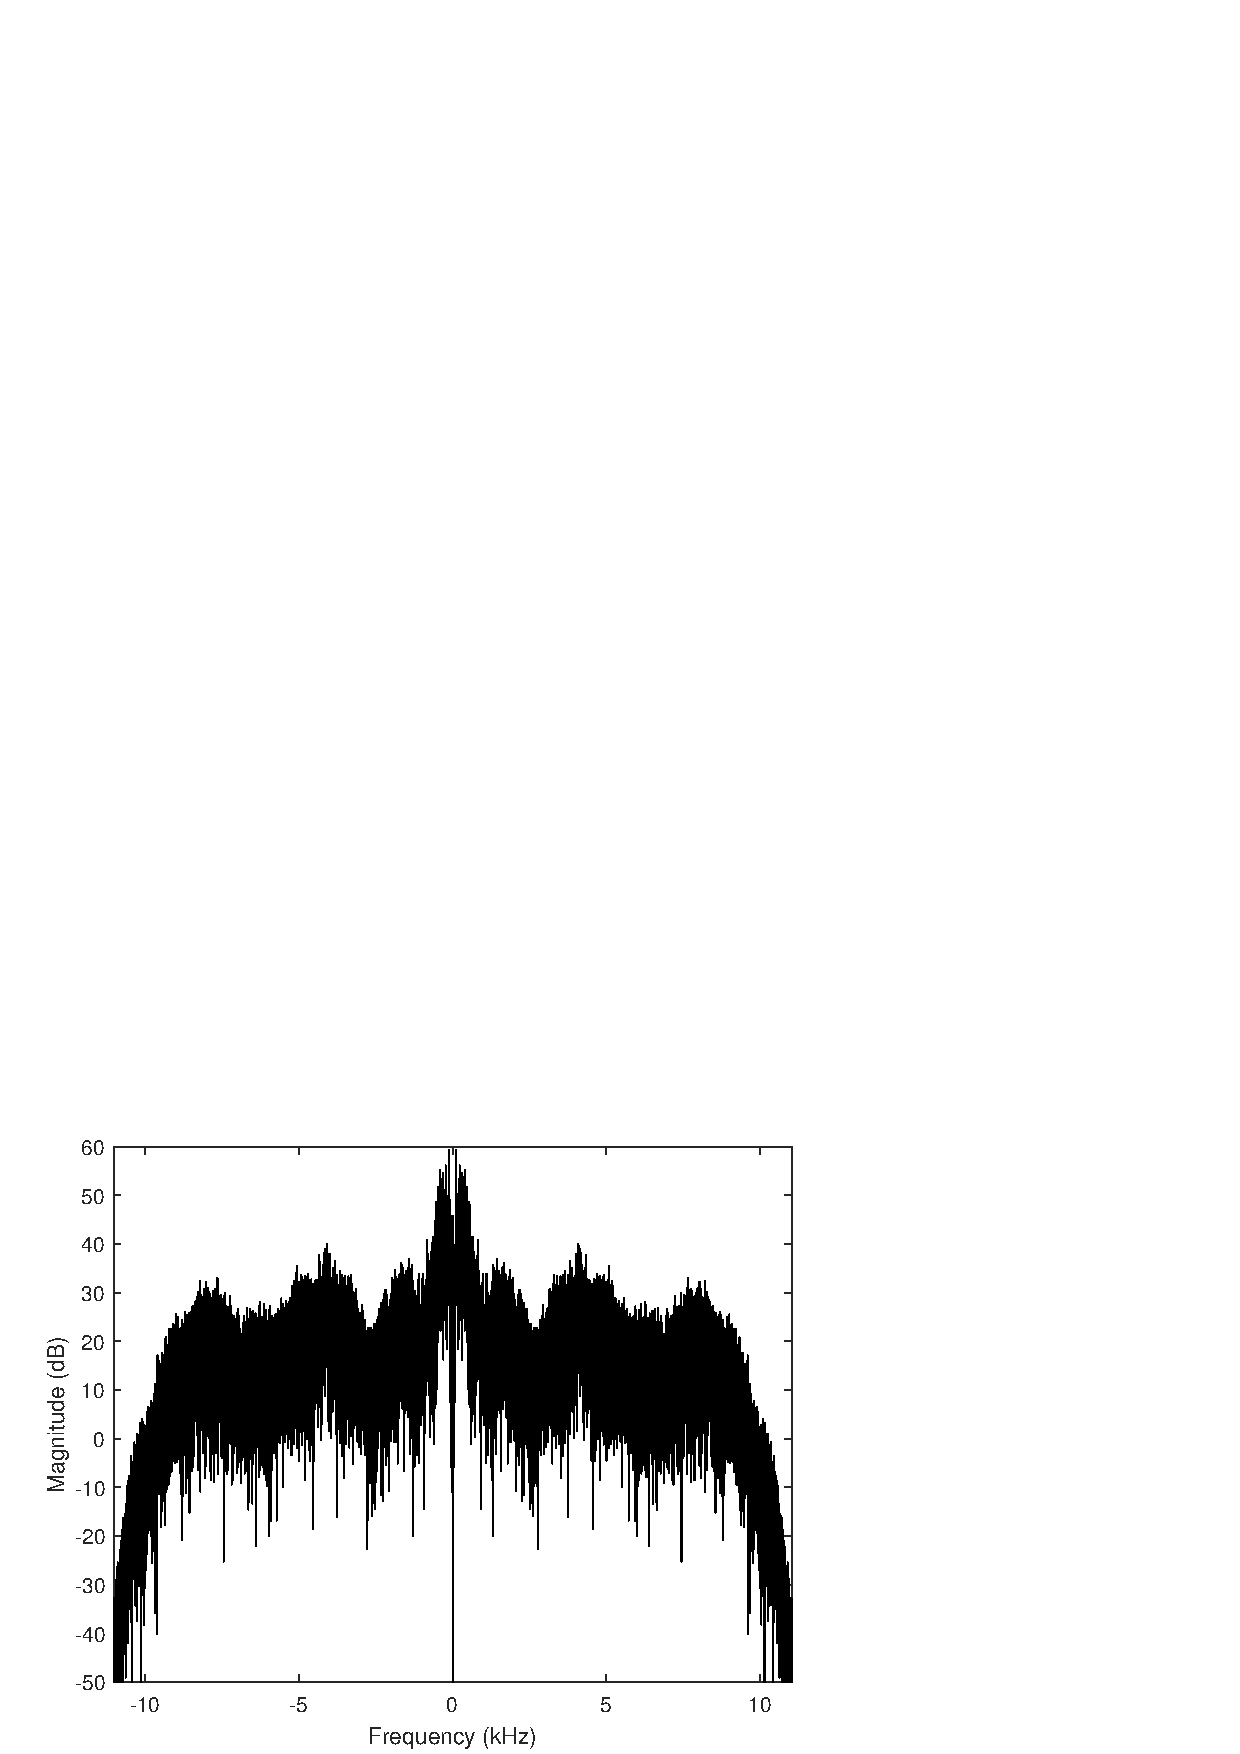
\includegraphics[scale=0.5]{figs/speech_dft_spectrum.png}
	\end{center}
	
	\begin{itemize}
		\item It has duration of about 4 seconds
		\item 110033 samples
		\item Not very informative. What are the main frequency components at the beginning of the third second?
	\end{itemize}
\end{frame}

%
\begin{frame}{Time-dependent Fourier transform (TDFT)}
\textbf{Time-dependent Fourier transform (TDFT)} or \textbf{short-time Fourier transform (STFT)} is defined as
\begin{equation*}
	X[n, \lambda) = \sum_{m = -\infty}^{\infty}x[n+m]w[m]e^{-j\lambda m}
\end{equation*}

\textbf{Notation:} $n$ is discrete, while $\lambda$ is continuous. This is why $n$ appears with a square bracket $[$ and $\lambda$ appears with parenthesis $)$.
\vspace{0.25cm}

If the window $w[n]$ has finite length $L$
\begin{equation*}
X[n, \lambda) = \sum_{m = 0}^{L-1}x[n+m]w[m]e^{-j\lambda m}
\end{equation*}

\end{frame}

%
\begin{frame}{Time-dependent Fourier transform (TDFT)}

Two interpretations for $X[n, \lambda)$:

\begin{enumerate}
	\item For fixed $n$, $X[n, \lambda)$ is the DTFT of $x[n+m]w[m]$. 
	\begin{equation}
		X[n, \lambda) = \mathcal{F}_\lambda\{x[n+m]w[m]\} \tag{fixed $n$}
	\end{equation}
	
	Hence, at fixed $n$, $X[n, \lambda)$ has all the properties of the DTFT.
	\vspace{0.25cm}
	\item For fixed $\lambda$, $X[n, \lambda)$ is the result of band-pass filtering the signal $x[n]$ by the time-reversed window $W(e^{-j\omega})$ centered at frequency $\lambda$
	
	\begin{align*}
		X[n, \lambda) &= \sum_{m = -\infty}^{\infty}x[n+m]w[m]e^{-j\lambda m} \tag{definition} \\
		&= \sum_{l = -\infty}^{\infty}x[l]w[-(n-l)]e^{j\lambda(n-l)} \tag{change of variables $l = n+m$} \\
		&=x[n]\ast h_\lambda[n] \tag{fixed $\lambda$}
	\end{align*}
	where 
	\begin{equation*}
		h_\lambda[n] = w[-n]e^{j\lambda n} \Longleftrightarrow H_\lambda(e^{j\omega}) = W(e^{-j(\omega-\lambda)}) 
	\end{equation*}
	
\end{enumerate}
\end{frame}

%
\begin{frame}{Sampling and displaying the TDFT: spectrograms}
	\textbf{Spectrogram} is a useful way of visualizing the TDFT
	
	Sampling both in time and frequency.
	We sample with period $R$ in time and with period $2\pi/N$ in frequency. $R$ is the block spacing and $N$ is the DFT length
	
	\begin{align}
		X[rR, k] &= X[rR, 2\pi k/N), \quad k = 0, \ldots, N-1 \tag{sample in time and frequency} \\
		&= \sum_{m = 0}^{L-1}x[rR+m]w[m]e^{-j(2\pi/N)km} \tag{finite-length window}
	\end{align}
			
	For fixed $r$, $X[rR, k]$ is the $N$-point DFT of $x[rR+m]w[m]$
	
\end{frame}

%
\begin{frame}{Sampling and displaying the TDFT: spectrograms}
Example using Kaiser window of length $L = 700$, FFT size $N = 700$, and $R = 550$.
\begin{center}
	\resizebox{0.9\textwidth}{!}{\begin{tikzpicture}
\begin{axis}[
	name=plot1,
	axis y line=middle, axis x line=bottom,
	enlargelimits = false, clip=false,
	scale only axis,
	width=\textwidth,
	height=0.2\textwidth,
	ymin=-0.6,	ymax=0.6,
	xmin={0}, xmax={200},
	axis line style={->,>=stealth},
	x axis line style={shorten >= -0.25cm}, 
	xlabel={\large $t$ (ms)},
	ylabel={\large $x(t)$},
	every axis x label/.style={
		at={(ticklabel* cs:1)},
		xshift=0.5cm,
		anchor=north west,
	},
	every axis y label/.style={
		at={(ticklabel* cs:1)},
		anchor=south,
	},
	xtick={50,100,...,200},
	xmajorgrids,
	ytick=\empty,
	extra x ticks={50,100,...,200},
	extra x tick labels={550, 1100,...,2200},
	every extra x tick/.style={major tick length=0pt,
	xtick align=outside,yshift=-15pt},
	every outer y axis line/.append style={white!15!black},
	every y tick label/.append style={font=\color{white!15!black}},
	legend style={draw=white!15!black,fill=white,legend cell align=left}]
	\node[below, anchor=north west, xshift=0.5cm,yshift=-15pt]  at (axis cs: 200,-0.6) {\large $n$ (samples)};
	
	\only<1-|handout:1->{
		\addplot [smooth, color=black, solid, line width=1pt] table[x index=0,y index=1] {figs/data/speech_sample.dat};
	}

	\only<2-|handout:2->{
		\addplot [smooth, color=blue2, solid, line width=1pt, restrict x to domain=0:63] table[x index=0,y index=1] {figs/data/speech_sample.dat};
	}

	\only<3-|handout:3->{
	\addplot [smooth, color=red2, solid, line width=1pt, restrict x to domain=50:113] table[x index=0,y index=1] {figs/data/speech_sample.dat};
	}

	\only<4-|handout:4->{
	\addplot [smooth, color=green2, solid, line width=1pt, restrict x to domain=100:163] table[x index=0,y index=1] {figs/data/speech_sample.dat};
	}

	\only<5-|handout:5->{
	\addplot [smooth, color=orange2, solid, line width=1pt, restrict x to domain=150:213] table[x index=0,y index=1] {figs/data/speech_sample.dat};
	}
	
\end{axis}

\begin{axis}[
name=plot2,
at=(plot1.below south east), anchor=above north east,
axis y line=middle, axis x line=bottom,
enlargelimits = false, clip=false,
scale only axis,
width=\textwidth,
height=0.2\textwidth,
%ymin=-0.6,	ymax=0.6,
xmin={0}, xmax={5.5},
axis line style={->,>=stealth},
x axis line style={shorten >= -0.25cm}, 
xlabel={\large Frequency (kHz)},
ylabel={\large dB},
every axis x label/.style={
	at={(ticklabel* cs:1)},
	xshift=0.5cm,
	anchor=north west,
},
every axis y label/.style={
	at={(ticklabel* cs:1)},
	anchor=south,
},
ymajorgrids,
xtick={0,..., 5},
every outer y axis line/.append style={white!15!black},
every y tick label/.append style={font=\color{white!15!black}},
legend style={draw=white!15!black,fill=white,legend cell align=left}]

\only<2|handout:2>{
	\addplot [smooth, color=blue2, solid, line width=1pt] table[x index=0,y index=4] {figs/data/speech_spectrogram_dft.dat};
}

\only<3|handout:3>{
	\addplot [smooth, color=red2, solid, line width=1pt] table[x index=0,y index=3] {figs/data/speech_spectrogram_dft.dat};
}

\only<4|handout:4>{
	\addplot [smooth, color=green2, solid, line width=1pt] table[x index=0,y index=2] {figs/data/speech_spectrogram_dft.dat};
}

\only<5|handout:5>{
	\addplot [smooth, color=orange2, solid, line width=1pt] table[x index=0,y index=1] {figs/data/speech_spectrogram_dft.dat};
}

\end{axis}

\onslide<2|handout:2>{
\node[anchor=north east] at ($(plot2.south east)+(0.8cm, -0.7cm)$) {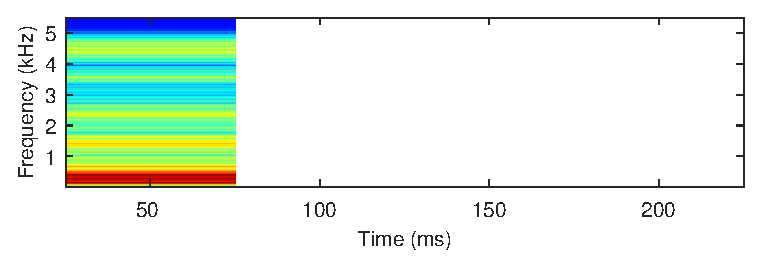
\includegraphics{figs/spectrogram_demo_pt1.eps}};
}

\onslide<3|handout:3>{
	\node[anchor=north east] at ($(plot2.south east)+(0.8cm, -0.7cm)$) {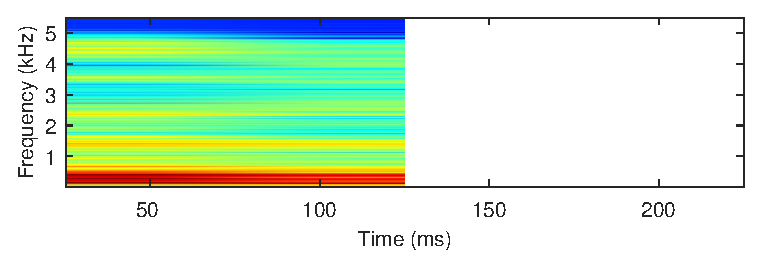
\includegraphics{figs/spectrogram_demo_pt2.eps}};
}

\onslide<4|handout:4>{
	\node[anchor=north east] at ($(plot2.south east)+(0.8cm, -0.7cm)$) {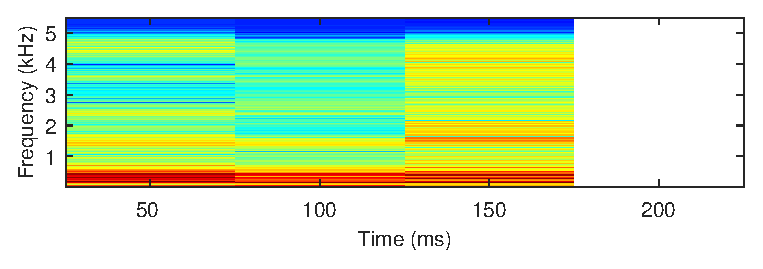
\includegraphics{figs/spectrogram_demo_pt3.eps}};
}

\onslide<5|handout:5>{
	\node[anchor=north east] at ($(plot2.south east)+(0.8cm, -0.7cm)$) {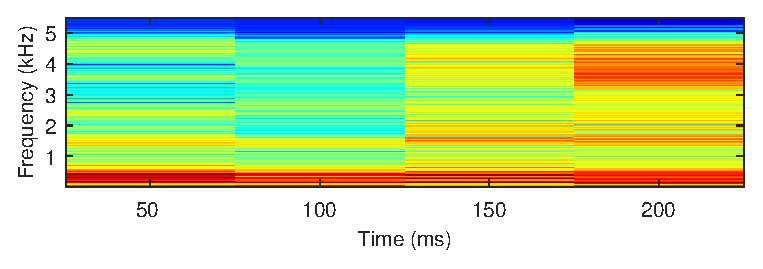
\includegraphics{figs/spectrogram_demo_pt4.eps}};
}

\end{tikzpicture}	
}
\end{center}
\end{frame}

\begin{frame}{Spectrogram in Matlab}
	To produce spectrogram plot
	\begin{align*}
		\texttt{>> spectrogram(x, window,noverlap,nfft)} \tag{Matlab notation}
	\end{align*}
	
	Using notation of this lecture notes:
	\begin{align*}
	\texttt{>> spectrogram(x, kaiser(L, beta), L-R, N)} \tag{this lecture's notation}
	\end{align*}
	The time blocks overlap by $L-R$ samples. Kaiser window was just as an example, any other window would work.
	
	\vspace{0.25cm}
	
	We can also use:
	\begin{align*}
		\texttt{>> [s,f,t] = spectrogram(x, kaiser(L, beta), L-R, N, fs)}
	\end{align*}
	This will not produce the plot, but it'll return the magnitude \texttt{s} in dB, the frequency vector \texttt{f} in Hz, and the time vector \texttt{t} in s.
\end{frame}

\begin{frame}{Spectrogram example}
	Spectrogram Canvas/Files/Matlab/\texttt{dft\_speech.wav}
	
	\begin{align*}
	&\texttt{>> spectrogram(x, kaiser(L=441, beta=6), R=220,...}\\
	&\texttt{ N = 441, Fs=22050, `yaxis')} 
	\end{align*}
	
	\begin{center}
		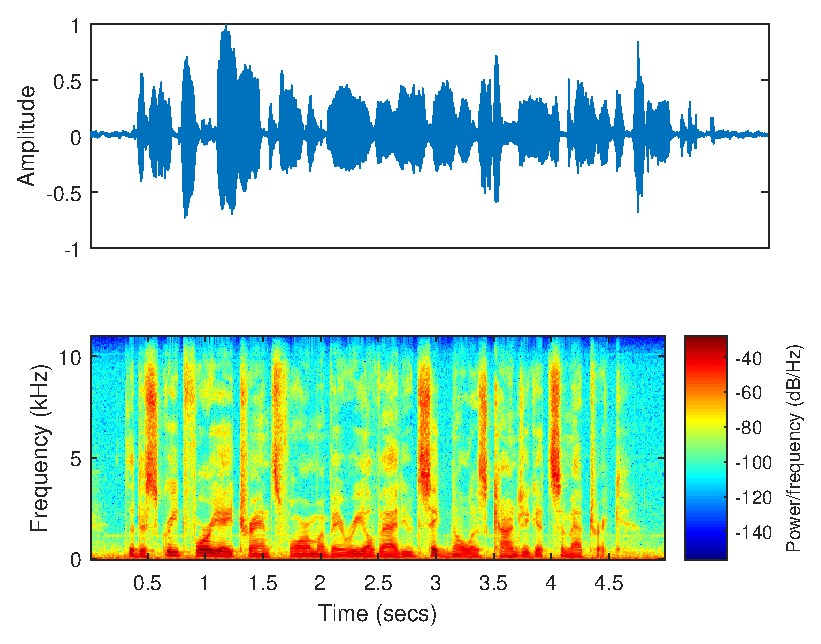
\includegraphics[scale=0.6]{figs/speech_spectogram_kaiser.eps}
	\end{center}
\end{frame}

\begin{frame}{Importance of window length}
Consider the following signal
\begin{align*}
	x[n] = \begin{cases}
	0, & n < 0 \\
	\cos(\alpha_0n^2), & 0 \leq n \leq 20000 \\
	\cos(0.2\pi n), & 20000 < n \leq 25000 \\
	\cos(0.2\pi n) + \cos(0.23\pi n), & n > 25000
	\end{cases}
\end{align*}

This signal has three sections
\begin{enumerate}
	\item linear chirp section. Frequency increases linearly
	\item Single tone at frequency $0.2\pi$
	\item Two tones: one at frequency $0.2\pi$ and another at $0.23\pi$
\end{enumerate}

\end{frame}


\begin{frame}{Importance of window length}
Spectrogram of $x[n]$ using the Hamming window of length 401 and 101.
\begin{center}
	\includegraphics[scale=0.7]{figs/spectrogram_window_length.png}
\end{center}

\textbf{Important:} window length determines the resolution.

\end{frame}

\begin{frame}{Inverting the TDFT}
We want to reconstruct $x[n]$ from its TDFT $X[n, \lambda)$:
\begin{equation*}
	x_r[n] = x[rR+n]w[n] = \frac{1}{N}\sum_{k = 0}^{N-1}X[rR, k]e^{j(2\pi/N)kn} \quad 0 \leq n \leq L-1
\end{equation*}

If the window is non-zero, we can divide it out to recover the signal $x[rR+n]$ over the window interval. If the windows overlap, we can recover all the original samples. This requires
\begin{equation*}
	R \leq L \leq N
\end{equation*}

The particular case when $R = L \leq N$ is called \textbf{maximally decimated condition}.

\end{frame}

\begin{frame}{Summary}
\begin{itemize}
	\item Leakage and resolution are important considerations in spectrum analysis
	\item By properly choosing windows we can minimize these issues
	\item Kaiser window is a nearly optimal choice. Must choose correct $\beta$ and window length $L$
	\item $\beta$ controls the ratio between the amplitudes of the main-lobe and the largest side-lobe i.e., $\beta$ controls the amount of leakage.
	\item The larger the main-lobe width, the smaller the resolution
	\item By increasing the window length we reduce the main-lobe width and consequently improve the resolution
	\item Time-dependent Fourier transform or short-time Fourier transform allows us to keep track of frequency variation in time
	\item Spectrogram is a commonly used way to display the TDFT
	\item In the spectrogram the TDFT is sampled both in time and in frequency
	\item The window length determines the resolution of the spectrogram
\end{itemize}
\end{frame}

\end{document}
